\documentclass[runningheads]{llncs}

\usepackage[T1]{fontenc}
\usepackage{amsmath,amssymb}
\usepackage{booktabs}
\usepackage{graphicx}
\usepackage{xcolor}
\usepackage{colortbl}
\usepackage{array}
\usepackage{url}
\usepackage[hidelinks]{hyperref}

\definecolor{tablerowalt}{RGB}{245,248,250}
\newcommand{\best}[1]{\textbf{#1}}

\setlength{\tabcolsep}{4pt}
\renewcommand{\arraystretch}{1.08}
\urlstyle{rm}
\emergencystretch=2em

\title{FRAA: A Retrieval-Augmented Agent for Explainable Financial Risk Assessment}
\titlerunning{FRAA for Financial Risk Assessment}

\author{}
\authorrunning{}
\institute{}

\begin{document}
\maketitle

\begin{abstract}
Financial risk assessment depends on probabilities that are well calibrated, sensitive to recent external evidence, and sufficiently transparent for human review. In many deployed settings, risk models still rely on manually engineered tabular features and tree ensembles. These models remain effective for stable feature stores, but they have limited access to long behavioral histories and to market or regulatory information that changes after training. This paper presents the Financial Risk Assessment Agent (FRAA), a retrieval-augmented model for explainable financial risk assessment. For each scoring request, FRAA encodes heterogeneous user behavior with a time-aware Transformer, retrieves timestamp-valid documents from a financial knowledge base, fuses the retrieved evidence through cross-attention, and outputs both a calibrated risk score and a concise textual justification. On a proprietary 24-month multi-source dataset with over 20 million users, 1.2 billion interactions, and 15 data sources, FRAA achieves a Log Loss of 0.5163 and Recall@5 of 0.4185. These results correspond to a 19.6\% Log Loss reduction relative to a deployed Random Forest baseline and a 9.4\% reduction relative to a non-retrieval Transformer. Ablation studies identify knowledge retrieval as the largest contributor, while retrieval-depth analysis shows that five retrieved documents provide the best trade-off between coverage and noise. Further evaluations cover cross-scenario adaptation, explanation quality rated 4.32/5 by domain experts, and 15.7 ms per-query latency under the tested serving configuration.

\keywords{Financial risk assessment \and Retrieval-augmented generation \and Explainable AI \and Risk scoring \and Time-aware Transformer}
\end{abstract}

\section{Introduction}

Financial institutions assess user-level risk from evidence that is heterogeneous, time-varying, and often incomplete at the moment of decision. Such evidence includes transaction histories, account states, macroeconomic indicators, regulatory disclosures, and news sentiment. Reliable risk estimates support credit review, fraud prevention, margin control, and compliance workflows \cite{hand1997statistical,thomas2000survey,crook2007recent,bolton2002statistical,ngai2011application}. In practice, many deployed systems still use carefully engineered tabular features with tree-based models such as Random Forests and gradient boosting \cite{breiman2001random,friedman2001greedy,chen2016xgboost,lessmann2015benchmarking}. These models remain strong operational baselines. However, their predictive state is usually fixed by the feature store, and they do not naturally incorporate long behavioral histories or newly released external information.

Neural sequence models and Transformer architectures offer a more flexible way to model user behavior over time \cite{hochreiter1997lstm,cho2014learning,vaswani2017attention,kang2018sasrec,sun2019bert4rec,jurgovsky2018sequence}. Yet a purely parametric sequence model remains limited in a financial risk setting. It can use market or regulatory information only if that information was encoded during training or manually attached as a feature. It also gives reviewers little direct evidence for why a high-risk case was flagged. Retrieval-augmented generation (RAG) and dense retrieval methods provide a way to condition decisions on external evidence available at inference time \cite{robertson2009probabilistic,karpukhin2020dpr,lewis2020rag,izacard2021leveraging}. In parallel, work on explanation and calibration has shown that model outputs need to be inspectable as well as accurate \cite{ribeiro2016lime,lundberg2017shap,guidotti2018survey,arrieta2020explainable,guo2017calibration,niculescu2005predicting,zadrozny2002transforming}. These observations motivate a risk model that retrieves time-valid financial evidence and links that evidence to both prediction and explanation.

This work develops the \textbf{Financial Risk Assessment Agent (FRAA)}, a retrieval-augmented model for explainable financial risk assessment. The word ``agent'' is used in a constrained operational sense. For each scoring request, FRAA builds a user state, queries a timestamped financial knowledge base, fuses retrieved evidence with behavioral features, estimates a risk probability, and generates a short explanation grounded in the retrieved context and influential feature groups. FRAA is therefore a structured retrieve-fuse-score-explain pipeline rather than an open-ended autonomous system.

The main contributions are:
\begin{itemize}
    \item We design a retrieval-augmented financial risk model that combines time-aware sequence encoding, external evidence retrieval, cross-attention evidence fusion, calibrated risk scoring, and explanation generation.
    \item We evaluate FRAA on a large-scale proprietary multi-source dataset with a strict chronological split, and compare it with deployed tree-based baselines and neural sequence models.
    \item We report component ablations, feature-group occlusion, retrieval-depth analysis, scenario adaptation, explanation quality assessment, and latency measurements to examine the contribution and operational cost of the retrieval and explanation components.
\end{itemize}

\section{Related Work}

\subsection{Financial Risk Modeling and Tabular Baselines}
Credit and financial risk prediction has long relied on statistical classifiers, scorecards, tree ensembles, support vector machines, and gradient boosting. These methods handle heterogeneous tabular features and have strong empirical performance across many credit-scoring studies \cite{hand1997statistical,thomas2000survey,baesens2003benchmarking,abdou2011credit,louzada2016classification,breiman2001random,friedman2001greedy,chen2016xgboost,lessmann2015benchmarking}. Prior work also shows that credit and fraud datasets are often imbalanced and operationally asymmetric, so ranking quality and calibration matter in addition to raw classification accuracy \cite{crook2007recent,brown2012experimental,khandani2010consumer,bellotti2009support,bolton2002statistical,ngai2011application}. In production, these models are commonly supported by feature stores and domain-specific aggregation rules. Their limitation is not weak performance on static tables, but the maintenance cost of hand-crafted features and the difficulty of using newly emerging external evidence at inference time.

\subsection{Sequential User Modeling}
Sequential recommendation and behavior modeling show that recurrent networks and Transformer encoders can capture evolving user states \cite{hochreiter1997lstm,cho2014learning,vaswani2017attention,kang2018sasrec,sun2019bert4rec}. Financial risk assessment has a related temporal structure. Recent transactions, account changes, and market signals form irregular sequences whose relevance depends on timing and context. Sequence models have also been applied to credit-card fraud detection, where temporal order is central to identifying abnormal behavior \cite{jurgovsky2018sequence}. FRAA follows this line of work but adapts it to calibrated risk scoring, where explanation is part of the target behavior rather than an optional post-processing step.

\subsection{Retrieval-Augmented and Explainable AI}
Dense retrieval and RAG methods condition model outputs on non-parametric external evidence \cite{robertson2009probabilistic,karpukhin2020dpr,lewis2020rag,izacard2021leveraging}. Text encoders such as BERT and Sentence-BERT provide practical document representations for semantic matching \cite{devlin2019bert,reimers2019sentence}. Approximate nearest-neighbor methods and vector search libraries such as Facebook AI Similarity Search (FAISS) make such retrieval feasible at large scale \cite{malkov2020hnsw,johnson2019billion}. In regulated domains, however, retrieval alone is not sufficient. Local explanation methods such as LIME and SHAP \cite{ribeiro2016lime,lundberg2017shap}, broader XAI surveys \cite{guidotti2018survey,arrieta2020explainable}, and calibration analyses \cite{guo2017calibration,niculescu2005predicting,zadrozny2002transforming} all point to the same requirement: a risk model should expose not only a probability, but also the evidence used to support it.

\section{Method}
\label{sec:method}

\subsection{Problem Formulation}
For a user $u$ and decision time $t$, the task is to estimate the probability $\hat{r}_t \in [0,1]$ that a material adverse event will occur within the next 30 days. The label $y_t \in \{0,1\}$ indicates whether such an event is observed. The model receives a time-ordered window of behavioral, profile, macroeconomic, and external-document signals available no later than $t$. This chronological constraint is applied throughout training and testing to avoid future information leakage.

Each training instance is built from an observation window ending at $t$ and a prediction window that immediately follows it. Dynamic events after $t$ are excluded. Slowly changing attributes are read from the latest snapshot available before $t$. External documents follow the same rule: a document can be retrieved only if its publication or ingestion timestamp is no later than the scoring time. This setup reflects operational risk review, where decisions are made before the adverse event and before later market information becomes available.

\subsection{Multi-Source State Construction}
FRAA maps the available evidence into three feature families. The dynamic transactional context $\mathbf{d}_t \in \mathbb{R}^{D_d}$ summarizes recent transaction amount, frequency, volatility, merchant category, and event timing. The quasi-static profile context $\mathbf{s}_t \in \mathbb{R}^{D_s}$ contains slowly changing user attributes, including account tenure, product holdings, balance ranges, and risk tier. The market and macro context $\mathbf{m}_t \in \mathbb{R}^{D_m}$ contains time-aligned external indicators available before the scoring time. The external-document branch is motivated by evidence that news and regulatory language can carry risk-relevant signals \cite{tetlock2007giving,loughran2011liability}.

Let $D_d$, $D_s$, and $D_m$ denote the dimensions of the three feature families. These vectors are concatenated and projected into a shared hidden space:
\begin{equation}
\mathbf{x}_t = \mathbf{W}_p [\mathbf{d}_t \Vert \mathbf{s}_t \Vert \mathbf{m}_t] + \mathbf{b}_p,
\label{eq:state_projection}
\end{equation}
where $\Vert$ denotes concatenation, $\mathbf{W}_p \in \mathbb{R}^{D_h \times (D_d+D_s+D_m)}$ and $\mathbf{b}_p \in \mathbb{R}^{D_h}$ are trainable parameters, and $\mathbf{x}_t \in \mathbb{R}^{D_h}$ is the initial user-state representation.

\subsection{Time-Aware Sequence Encoding}
Financial behavior is observed at irregular intervals. FRAA therefore injects a time-gap encoding into each event representation. Let $\Delta \tau_i$ denote the elapsed time between consecutive events. The input to layer $l$ of the Transformer encoder is updated as
\begin{equation}
\mathbf{h}_i^{(l)} =
\mathrm{TransformerBlock}^{(l)}\left(\mathbf{h}_i^{(l-1)} + \mathbf{p}_{\Delta \tau_i}\right),
\quad l=1,\ldots,L,
\label{eq:time_transformer}
\end{equation}
where $\mathbf{p}_{\Delta \tau_i}$ is the time-gap embedding. The final state $\mathbf{h}_t^{(L)}$ summarizes the user's observed behavior up to time $t$.

\subsection{Retrieval-Augmented Evidence Fusion}
\label{sec:retrieval}
To incorporate external knowledge, FRAA converts the encoded user state into a retrieval query:
\begin{equation}
\mathbf{q}_t = f_q(\mathbf{h}_t^{(L)}),
\label{eq:query}
\end{equation}
where $f_q(\cdot)$ is a lightweight multilayer perceptron that maps the sequence state to the document-embedding space. The financial knowledge base contains approximately 1.2 million timestamped documents, including regulatory filings, market reports, news articles, and macroeconomic commentaries. Documents are embedded offline and indexed with FAISS. At inference time, FRAA retrieves the top-$K$ documents by cosine similarity:
\begin{equation}
\mathcal{D}_t =
\operatorname{topK}_{d \in \mathcal{K}_t}
\frac{\mathbf{q}_t^\top \mathbf{e}_d}{\|\mathbf{q}_t\|\|\mathbf{e}_d\|},
\label{eq:retrieval}
\end{equation}
where $\mathcal{K}_t$ contains only documents available no later than $t$, and $\mathbf{e}_d$ is the embedding of document $d$. Document embeddings are produced by a financial-domain text encoder initialized from bidirectional Transformer encoders and sentence-level retrieval models \cite{devlin2019bert,reimers2019sentence}. The timestamp restriction prevents future documents from leaking into the prediction.

The retrieved document embeddings are fused with the user state using cross-attention:
\begin{equation}
\tilde{\mathbf{h}}_t =
\mathrm{CrossAttn}
\left(
\mathbf{h}_t^{(L)}\mathbf{W}_Q,
\mathbf{D}_t\mathbf{W}_K,
\mathbf{D}_t\mathbf{W}_V
\right),
\label{eq:cross_attention}
\end{equation}
where $\mathbf{D}_t \in \mathbb{R}^{K \times D_e}$ stacks the embeddings of retrieved documents, $D_e$ is the document-embedding dimension, and $\mathbf{W}_Q$, $\mathbf{W}_K$, and $\mathbf{W}_V$ are trainable projection matrices. The fused representation $\tilde{\mathbf{h}}_t$ is passed to the scoring and explanation heads. Cross-attention is used instead of simple concatenation because the relevance of external evidence depends on the user state. For example, a macroeconomic commentary may matter for users with concentrated sector exposure, but may be weakly relevant for users whose recent transactions do not involve that sector.

\subsection{Risk Scoring and Explanation Generation}
The risk head maps the fused representation to a calibrated probability:
\begin{equation}
\hat{r}_t = \sigma(\mathbf{w}_r^\top \tilde{\mathbf{h}}_t + b_r).
\label{eq:risk_score}
\end{equation}
where $\sigma(\cdot)$ is the sigmoid function, $\mathbf{w}_r$ is a trainable risk-head vector, and $b_r$ is a scalar bias. In parallel, the explanation head generates a concise textual justification from the retrieved documents and feature-group importance signals. The training objective combines per-instance binary cross-entropy for risk prediction with a supervised explanation-fidelity term:
\begin{equation}
\mathcal{L} =
-y_t \log \hat{r}_t - (1-y_t)\log(1-\hat{r}_t)
+ \lambda \mathcal{L}_{\mathrm{exp}}(\hat{e}_t, e_t^{\mathrm{ref}}),
\label{eq:loss}
\end{equation}
where $\hat{e}_t$ is the generated explanation, $e_t^{\mathrm{ref}}$ is an expert or rule-supported reference explanation, $\mathcal{L}_{\mathrm{exp}}$ penalizes mismatches with reference evidence and feature-group rationales, and $\lambda$ balances prediction and explanation supervision. The explanation head is trained to refer to retrieved evidence and influential feature groups, rather than to produce a free-form rationale disconnected from the risk score. In all reported experiments, the Transformer uses 8 attention blocks, hidden dimension 256, and embedding dimension 512. Retrieval depth is $K=5$ unless otherwise stated.

\begin{figure}
\centering
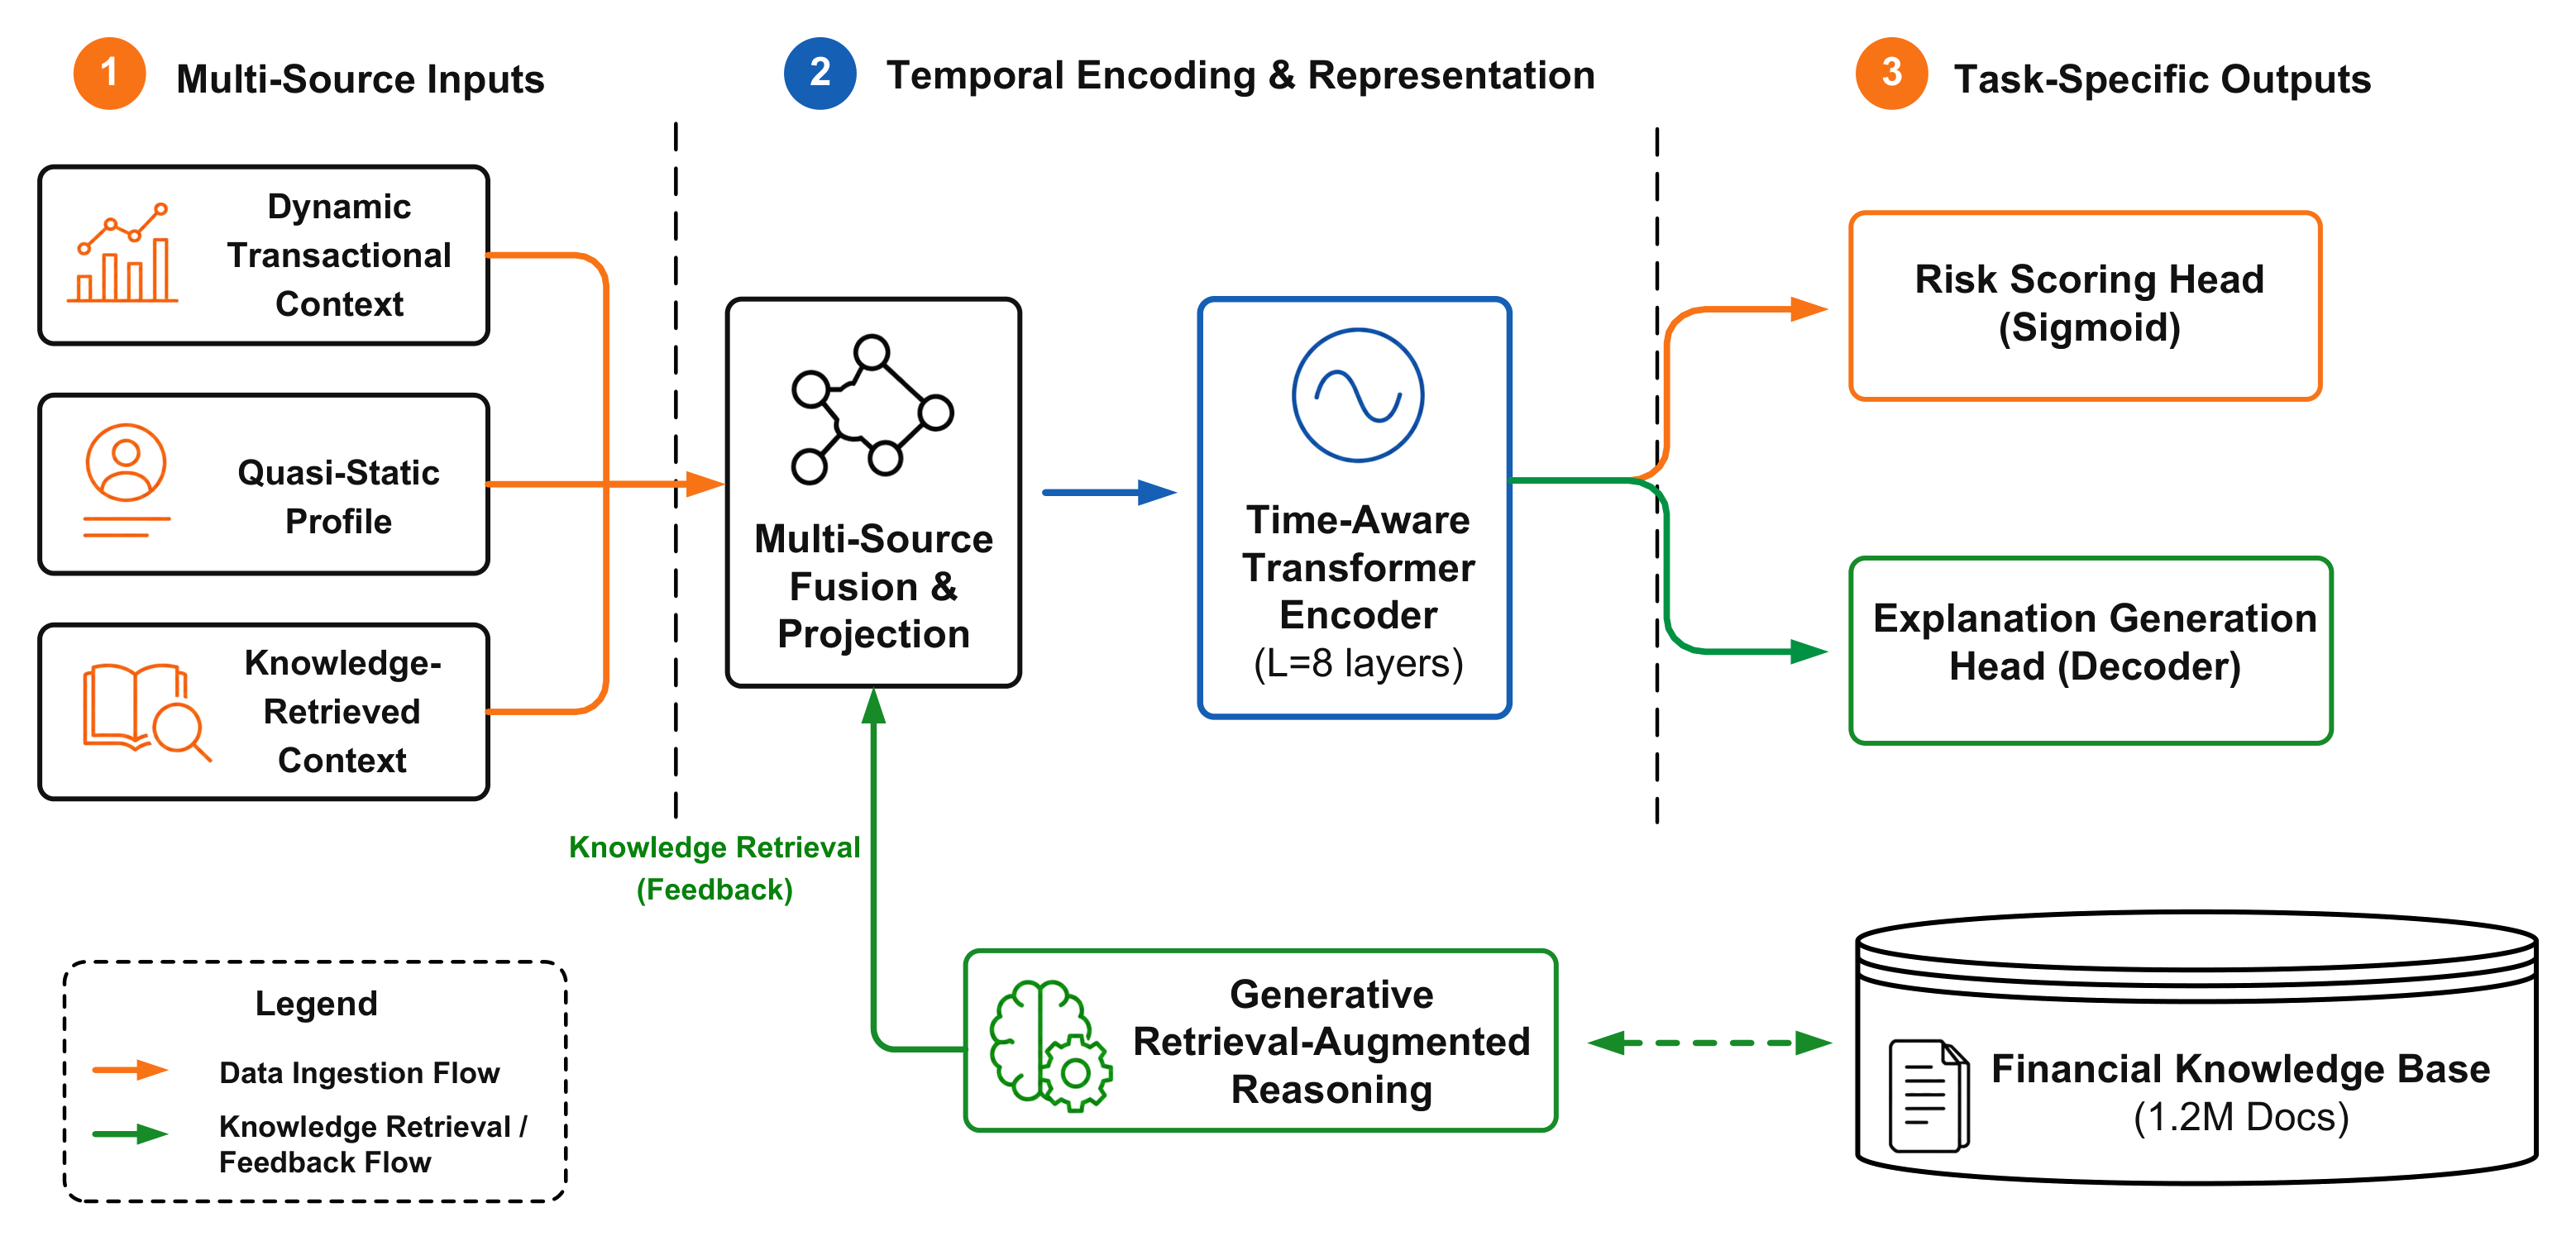
\includegraphics[width=0.88\textwidth]{figures/algorithm/algorithm_1_0ebe5141.png}
\caption{Overview of FRAA. The model encodes multi-source financial behavior, retrieves timestamp-valid documents from a financial knowledge base, fuses retrieved evidence with the user state, and outputs both a calibrated risk score and an explanation.}
\label{fig:algorithm}
\end{figure}

Figure~\ref{fig:algorithm} summarizes the inference path from multi-source evidence encoding to retrieval, fusion, scoring, and explanation generation.

\section{Experiments}
\label{sec:experiments}

\subsection{Dataset and Evaluation Protocol}
The dataset is a proprietary 24-month multi-source corpus from a financial risk environment. It contains over 20 million users, 1.2 billion interactions, and 15 heterogeneous data sources. Records include transaction events, account status snapshots, product holdings, macroeconomic series, and timestamped news or regulatory signals. The target indicates whether a material adverse event, such as default, severe delinquency, or forced liquidation, occurs within the next 30 days.

We use a strict chronological split. Historical records are used to build lookback features and timestamp-valid knowledge-base entries. The model is trained on a 12-month period, tuned on the following month, and evaluated on the final month. No validation or test-period documents are made available to earlier predictions. We report Log Loss for probability calibration, Recall@1/Recall@5 for risk-review ranking, area under the receiver operating characteristic curve (AUC) for feature-group occlusion, and longest common subsequence ROUGE (ROUGE-L) for explanation overlap with expert-written references.

The evaluation protocol follows the main failure modes of financial risk systems. Log Loss measures whether predicted probabilities are useful for downstream thresholding and risk appetite control. Recall@1 and Recall@5 measure the ranking quality of the highest-risk cases, which are the cases most likely to be reviewed by analysts. The chronological split and timestamp-valid retrieval rule are used for every model variant, including ablations, so that performance differences do not arise from different access to future information.

\subsection{Baselines and Training Details}
We compare FRAA with a deployed Random Forest (RF), RF with static knowledge-base (KB) features, XGBoost, LSTM, and a non-retrieval Transformer. These baselines cover the main operational choices in the target setting: tabular ensembles, tabular ensembles with manually attached external features, recurrent sequence modeling, and neural sequence modeling without retrieval. We retain the deployed tree-based baseline because prior credit-scoring and tabular-learning studies repeatedly find tree ensembles difficult to displace on heterogeneous tabular data \cite{baesens2003benchmarking,brown2012experimental,arik2021tabnet}. All baselines use the same chronological split and available feature families. FRAA is implemented in PyTorch and trained with AdamW, learning rate $1\times10^{-4}$, weight decay $1\times10^{-5}$, batch size 64, and a maximum budget of 50 epochs. The selected checkpoint is the one with the lowest validation Log Loss.

Hyperparameters are chosen on the validation month and then fixed for the test month. For retrieval variants, document embeddings are constructed offline and indexed before evaluation. During scoring, the retrieval pool is filtered by timestamp before nearest-neighbor search. This step is essential because a high-capacity retrieval model could otherwise use documents that were unavailable when the decision should have been made.

\subsection{Evaluation Questions}
The experiments address four questions. First, does retrieval-augmented evidence change calibrated risk prediction and high-risk ranking relative to tree-based and neural baselines? Second, do the learned representations transfer to related financial scenarios, or are they tied to a single product-specific task? Third, which components account for the observed gains, especially the dynamic transaction encoder, time-gap encoding, and knowledge retrieval module? Fourth, are the explanations and latency compatible with analyst-facing risk review? The following sections follow this order, separating the main predictive result from auxiliary analyses.

\subsection{Main Results}

We first compare the full model with deployed and neural baselines under the same chronological split. Table~\ref{tab:main_results} reports the numerical results, and Fig.~\ref{fig:main_results} visualizes the two primary metrics. The ordering is consistent across calibration and ranking: the full retrieval-augmented model outperforms tree-based baselines, the non-retrieval Transformer, and all ablated FRAA variants.

\begin{table}[!ht]
\centering
\caption{Main test-set performance. Lower Log Loss and higher Recall@5 are better.}
\label{tab:main_results}
\begin{tabular}{lcc}
\toprule
\textbf{Model} & \textbf{Log Loss} & \textbf{Recall@5} \\
\midrule
RF (deployed baseline) & 0.6421 & 0.3172 \\
\rowcolor{tablerowalt}
RF + KB features & 0.6289 & 0.3291 \\
XGBoost & 0.6104 & 0.3495 \\
\rowcolor{tablerowalt}
LSTM & 0.5873 & 0.3738 \\
Transformer & 0.5698 & 0.3846 \\
\rowcolor{tablerowalt}
FRAA (-Dyn) & 0.5642 & 0.3891 \\
FRAA (-TE) & 0.5510 & 0.3957 \\
\rowcolor{tablerowalt}
FRAA (-KB) & 0.5385 & 0.4023 \\
\textbf{FRAA (full)} & \best{0.5163} & \best{0.4185} \\
\bottomrule
\end{tabular}
\end{table}

Relative to the deployed RF baseline, FRAA reduces Log Loss by 19.6\% and raises Recall@5 from 0.3172 to 0.4185. Relative to the non-retrieval Transformer, it reduces Log Loss by 9.4\% and raises Recall@5 by 8.8\%. The ablated variants remain below the full model, indicating that retrieval, temporal encoding, and dynamic features contribute complementary information.

\begin{figure}[!ht]
\centering
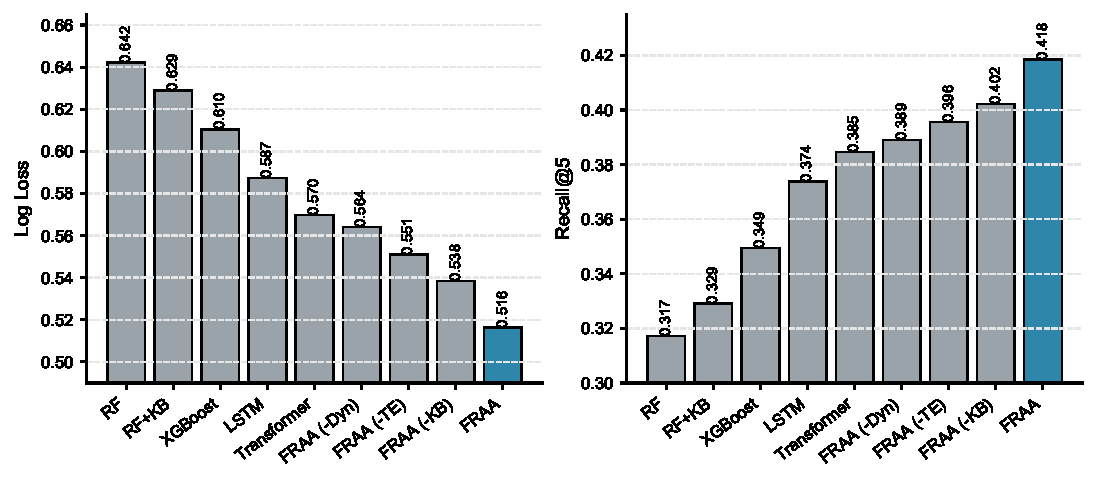
\includegraphics[width=0.86\textwidth]{figures/main_result/main_results_comparison.pdf}
\caption{Main-result comparison. FRAA obtains the lowest Log Loss and highest Recall@5 among all evaluated models.}
\label{fig:main_results}
\end{figure}

\subsection{Scenario Adaptation}

We then test whether representations learned from the multi-source corpus can be adapted to related risk scenarios with different product distributions.

\begin{table}
\centering
\caption{Cross-scenario adaptation measured by relative Recall lift over scenario-specific baselines.}
\label{tab:adaptation}
\begin{tabular}{lcc}
\toprule
\textbf{Adaptation method} & \textbf{Credit card R@1 / R@5} & \textbf{Mortgage R@1 / R@5} \\
\midrule
Scenario-specific model & 0.00 / 0.00 & 0.00 / 0.00 \\
\rowcolor{tablerowalt}
LP-FT ($<1\%$ params) & +3.14 / +2.97 & +2.88 / +2.45 \\
LoRA-FT ($<5\%$ params) & +13.49 / +12.63 & +11.72 / +10.88 \\
\rowcolor{tablerowalt}
\textbf{FRAA full-FT} & \best{+18.21 / +17.10} & \best{+16.45 / +15.33} \\
\bottomrule
\end{tabular}
\end{table}

Table~\ref{tab:adaptation} examines transfer to related financial scenarios. Linear-probe fine-tuning (LP-FT) updates only a small prediction layer, low-rank adaptation fine-tuning (LoRA-FT) updates low-rank adapter parameters \cite{hu2022lora}, and full fine-tuning (full-FT) updates the full model. Full-FT gives the largest gains, while LoRA-FT retains much of the benefit with fewer updated parameters. This pattern suggests that FRAA learns risk representations that can be reused across products, rather than only fitting a single product-specific task.

\section{Ablation and Analysis}
\label{sec:ablation}

\subsection{Architectural Components}
The component ablation removes one design choice at a time while keeping the training split, feature availability, and evaluation metrics unchanged. This setup separates the effect of retrieval from the effect of stronger sequence modeling.

\begin{table}
\centering
\caption{Component ablation on the risk-score prediction task.}
\label{tab:component_ablation}
\begin{tabular}{lcc}
\toprule
\textbf{Model variant} & \textbf{Log Loss} & \textbf{Recall@5} \\
\midrule
Transformer & 0.5698 & 0.3846 \\
\rowcolor{tablerowalt}
FRAA (-Dyn) & 0.5642 & 0.3891 \\
FRAA (-TE) & 0.5510 & 0.3957 \\
\rowcolor{tablerowalt}
FRAA (-KB) & 0.5385 & 0.4023 \\
\textbf{FRAA (full)} & \best{0.5163} & \best{0.4185} \\
\bottomrule
\end{tabular}
\end{table}

Table~\ref{tab:component_ablation} isolates the contribution of dynamic transactions (-Dyn), temporal encoding (-TE), and knowledge retrieval (-KB). Removing the knowledge component causes the largest degradation among FRAA variants: Log Loss increases from 0.5163 to 0.5385, and Recall@5 decreases from 0.4185 to 0.4023. This result supports the retrieval-augmented design. Removing temporal encoding also reduces performance, which is consistent with the irregular timing of financial events. The -Dyn variant remains stronger than the non-retrieval Transformer. External evidence and temporal encoding therefore compensate for some missing dynamic transaction information, but they do not replace it.

\subsection{Feature Groups and Retrieval Depth}
We next examine the gain from two complementary views: feature-family occlusion and retrieval depth.

\begin{table}
\centering
\caption{Feature-group occlusion. A larger AUC drop indicates a more important feature family.}
\label{tab:feature_occlusion}
\begin{tabular}{lc}
\toprule
\textbf{Occluded feature group} & \textbf{AUC drop (\%)} \\
\midrule
Knowledge-retrieved context & 3.92 \\
\rowcolor{tablerowalt}
Transaction dynamics & 2.87 \\
Macroeconomic indicators & 1.55 \\
\rowcolor{tablerowalt}
Quasi-static profile & 0.93 \\
\bottomrule
\end{tabular}
\end{table}

The occlusion results in Table~\ref{tab:feature_occlusion} are consistent with the component ablation. Knowledge-retrieved context produces the largest AUC drop, followed by transaction dynamics. Static profile variables still contribute, but they are less influential than time-sensitive behavioral and external-evidence signals. This ordering indicates that much of the model's advantage comes from information that changes over time rather than from static attributes alone.

\begin{table}
\centering
\caption{Effect of retrieval depth $K$.}
\label{tab:retrieval_depth}
\begin{tabular}{lcc}
\toprule
\textbf{Top-$K$ documents} & \textbf{Log Loss} & \textbf{Recall@5} \\
\midrule
1 & 0.5287 & 0.4068 \\
\rowcolor{tablerowalt}
3 & 0.5214 & 0.4117 \\
\textbf{5} & \best{0.5163} & \best{0.4185} \\
\rowcolor{tablerowalt}
7 & 0.5175 & 0.4173 \\
10 & 0.5189 & 0.4160 \\
\bottomrule
\end{tabular}
\end{table}

Table~\ref{tab:retrieval_depth} indicates that retrieval depth has a clear optimum in this setting. One or three documents provide insufficient external context. Seven or ten documents slightly degrade both metrics. We therefore use $K=5$ in the main experiments. The degradation at larger $K$ is small, but it is consistent with the retrieval-noise trade-off: broader retrieval increases coverage while introducing less relevant documents into the fusion module.

\section{Further Evaluation}

\subsection{Explanation Quality}
Beyond risk scores, FRAA is intended to support human review by explaining why a high-risk case was flagged. We therefore evaluate the generated explanations using both expert ratings and lexical overlap with reference explanations.

\begin{table}
\centering
\caption{Human and automatic evaluation of generated explanations. Higher scores are better.}
\label{tab:explanation_quality}
\begin{tabular}{lccc}
\toprule
\textbf{Method} & \textbf{Faithfulness} & \textbf{Readability} & \textbf{ROUGE-L} \\
\midrule
Template-based top-3 groups & 3.89 & 4.02 & 0.3026 \\
\rowcolor{tablerowalt}
\textbf{FRAA (full)} & \best{4.32} & \best{4.51} & \best{0.4131} \\
\bottomrule
\end{tabular}
\end{table}

Five domain experts evaluated 1,000 high-risk test predictions. Table~\ref{tab:explanation_quality} reports higher faithfulness, readability, and ROUGE-L for FRAA than for a template baseline that lists the top three feature groups. The result suggests that the explanation head adds information beyond feature enumeration. The expert ratings should be interpreted as an auditability signal, not as evidence that generated text is sufficient for automatic decision making.

\subsection{Latency and Offline Business Utility}
The final evaluation asks whether the added retrieval and fusion steps are practical for an analyst-facing review loop, and whether the calibration gain translates into offline decision-support utility.

\begin{table}
\centering
\caption{Inference latency and throughput under the tested batch-size-64 serving configuration.}
\label{tab:latency}
\begin{tabular}{lcc}
\toprule
\textbf{Model} & \textbf{Latency (ms/query)} & \textbf{Throughput (queries/s)} \\
\midrule
RF + KB features & 1.9 & 12,530 \\
\rowcolor{tablerowalt}
XGBoost & 2.1 & 11,200 \\
LSTM & 8.3 & 5,910 \\
\rowcolor{tablerowalt}
Transformer & 12.4 & 4,320 \\
\textbf{FRAA (full)} & 15.7 & 4,070 \\
\bottomrule
\end{tabular}
\end{table}

FRAA is slower than tree ensembles because it performs retrieval and neural sequence encoding. Even so, the tested latency in Table~\ref{tab:latency} remains compatible with interactive risk review. The retrieval step accounts for approximately 4.2 ms of the total latency. Throughput is lower than for tabular baselines, but remains above the level required for batched offline scoring and analyst triage in the tested configuration.

\begin{table}
\centering
\caption{Offline replay analysis of risk-adjusted revenue (RAR) utility.}
\label{tab:business}
\begin{tabular}{lcc}
\toprule
\textbf{Model} & \textbf{Log Loss reduction (\%)} & \textbf{RAR lift (\%)} \\
\midrule
RF + KB features & -2.06 & +1.89 \\
\rowcolor{tablerowalt}
Transformer & -11.26 & +5.34 \\
FRAA (-KB) & -16.13 & +7.80 \\
\rowcolor{tablerowalt}
\textbf{FRAA (full)} & \best{-19.59} & \best{+10.45} \\
\bottomrule
\end{tabular}
\end{table}

The offline replay in Table~\ref{tab:business} connects calibration with downstream utility under a fixed risk-appetite constraint. We report this as offline decision-support evidence, not as a claim of causal online revenue impact. The analysis checks whether lower Log Loss corresponds to a practically meaningful ordering of cases under a fixed review budget.

\section{Limitations and Reproducibility}

The evaluation uses a proprietary financial dataset that cannot be publicly released because it contains sensitive user-level risk and transaction information. This limits independent replication. To support reproducibility within this constraint, we report the data scale, feature families, chronological split, training configuration, retrieval depth, baselines, and ablation settings. The knowledge base is timestamped, and retrieval uses only documents available at or before the scoring time. These details make the experimental protocol auditable even when the raw records cannot be shared.

Several claims should be read within this scope. First, the results establish performance in one large multi-source financial environment, not universal transfer across institutions. Second, the business-utility analysis is based on offline replay and should not be interpreted as causal online impact evidence. Third, the current evaluation does not report multi-seed variance or formal statistical significance tests because the available audit record contains one fixed proprietary chronological split rather than repeated independent training runs. Fourth, the explanation evaluation measures expert-perceived faithfulness and readability for high-risk test predictions. It does not remove the need for human oversight in regulated decisions. Future work should add public benchmark evaluations where legally possible, repeatability analysis under multiple splits or random seeds, institution-level transfer tests, and governance mechanisms for retrieved evidence that may become outdated or disputed.

\section{Conclusion}

This paper presented FRAA, a retrieval-augmented model for explainable financial risk assessment. FRAA combines time-aware sequence modeling, timestamp-valid knowledge retrieval, cross-attention evidence fusion, calibrated risk scoring, and explanation generation. On a large-scale proprietary multi-source dataset, FRAA achieves the lowest Log Loss and highest Recall@5 among the evaluated models. Ablations identify knowledge retrieval as the most influential component, and retrieval-depth analysis selects five documents as the best trade-off between evidence coverage and noise. Additional evaluations examine cross-scenario transfer, explanation quality, and tested latency. Taken together, the results suggest that external evidence retrieval is most valuable when it is constrained by time validity, fused with temporal user behavior, and exposed through auditable explanations.

\bibliographystyle{splncs04}
\bibliography{submission_pricai2026}

\end{document}

